\documentclass{article}

\usepackage{multirow}
\usepackage{booktabs}
\usepackage{graphicx}
\usepackage[margin=0.5in]{geometry}

\begin{document}

\begin{figure}
  \centering
  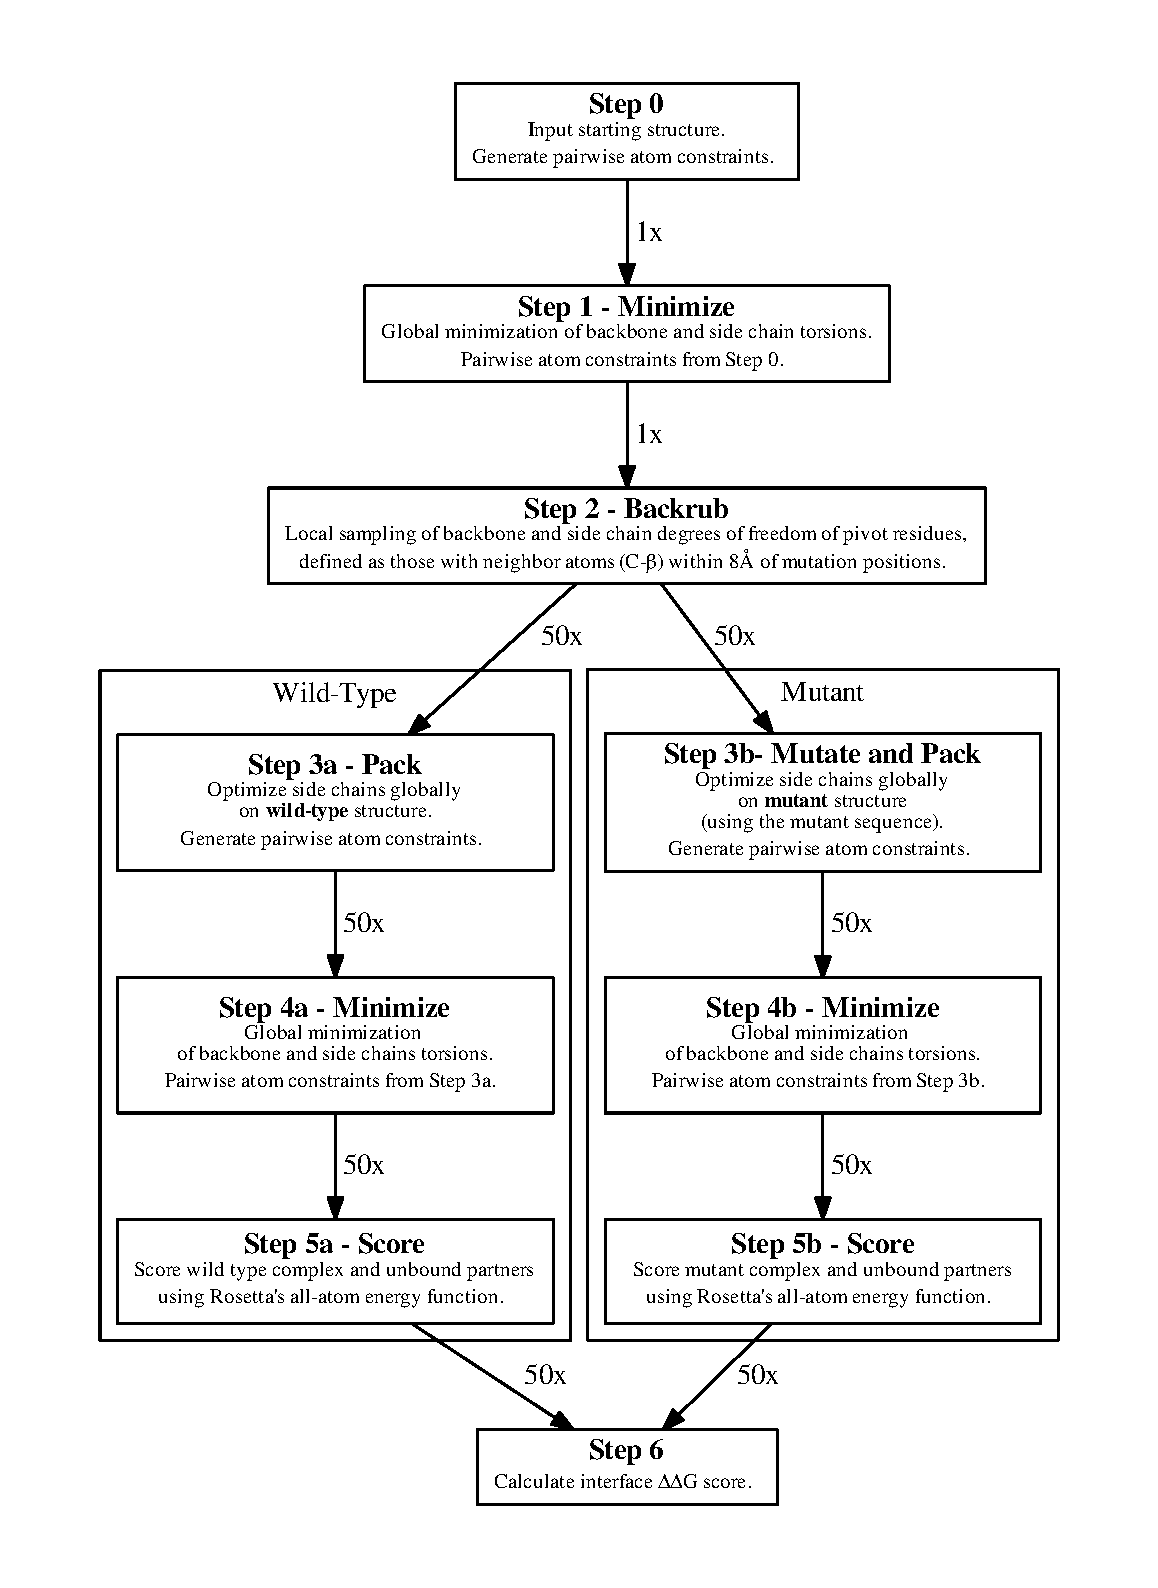
\includegraphics[width=\textwidth,keepaspectratio]{../../figures/fig-overview.pdf}
    \caption{
      Schematic of the flex ddG protocol method.
  } \label{fig:figure-overview}
\end{figure}

\begin{table}
  \begin{tabular}{rl}
\toprule
    n &                              Name \\
\midrule
 1240 &                  Complete dataset \\
  748 &        Single mutation to alanine \\
  273 &                Multiple mutations \\
  130 &        Small-to-large mutation(s) \\
   45 &  Multiple mutations, none alanine \\
\bottomrule
\end{tabular}

  \caption[]{ZEMu dataset subset definition and composition} \label{tab:table-composition}
\end{table}

\begin{table}
  \begin{tabular}{llrrrr}
\toprule
Mutation Category &   Prediction Method &     N &    R &  MAE &   FC \\
\midrule
 \multirow{ 4}{*}{Complete dataset} & flex ddG & \multirow{ 4}{*}{1240} & \textbf{0.63} & \textbf{0.96} & \textbf{0.76}  \\
 & ddG monomer & & 0.51 & 1.57 & 0.64  \\
 & no backrub control & & 0.57 & 1.12 & 0.73  \\
 & ZEMu paper & & 0.61 & 1.08 & 0.71  \\
\hline
 \multirow{ 4}{*}{Small-to-large mutation(s)} & flex ddG & \multirow{ 4}{*}{130} & \textbf{0.65} & \textbf{0.78} & \textbf{0.71}  \\
 & ddG monomer & & 0.31 & 1.55 & 0.55  \\
 & no backrub control & & 0.41 & 1.09 & 0.62  \\
 & ZEMu paper & & 0.48 & 1.16 & 0.65  \\
\hline
 \multirow{ 4}{*}{Mutation(s) to alanine} & flex ddG & \multirow{ 4}{*}{939} & \textbf{0.62} & \textbf{0.96} & \textbf{0.78}  \\
 & ddG monomer & & 0.50 & 1.55 & 0.66  \\
 & no backrub control & & 0.58 & 1.06 & 0.76  \\
 & ZEMu paper & & \textbf{0.62} & 1.03 & 0.73  \\
\hline
 \multirow{ 4}{*}{Single mutation to alanine} & flex ddG & \multirow{ 4}{*}{748} & \textbf{0.51} & \textbf{0.75} & \textbf{0.76}  \\
 & ddG monomer & & 0.36 & 1.31 & 0.62  \\
 & no backrub control & & 0.44 & 0.90 & 0.74  \\
 & ZEMu paper & & 0.45 & 0.86 & 0.71  \\
\hline
 \multirow{ 4}{*}{Multiple mutations} & flex ddG & \multirow{ 4}{*}{273} & 0.62 & \textbf{1.62} & \textbf{0.78}  \\
 & ddG monomer & & 0.50 & 2.44 & 0.70  \\
 & no backrub control & & 0.59 & 1.74 & 0.71  \\
 & ZEMu paper & & \textbf{0.64} & 1.63 & 0.75  \\
\hline
 \multirow{ 4}{*}{Multiple mutations, all to alanine} & flex ddG & \multirow{ 4}{*}{191} & 0.47 & 1.77 & \textbf{0.84}  \\
 & ddG monomer & & 0.34 & 2.49 & 0.80  \\
 & no backrub control & & 0.51 & \textbf{1.70} & 0.81  \\
 & ZEMu paper & & \textbf{0.55} & 1.72 & 0.79  \\
\hline
 \multirow{ 4}{*}{Multiple mutations, none to alanine} & flex ddG & \multirow{ 4}{*}{45} & \textbf{0.63} & \textbf{1.38} & \textbf{0.60}  \\
 & ddG monomer & & 0.40 & 2.54 & 0.38  \\
 & no backrub control & & 0.47 & 1.63 & 0.53  \\
 & ZEMu paper & & 0.53 & 1.59 & \textbf{0.60}  \\
\hline
 \multirow{ 4}{*}{Antibodies} & flex ddG & \multirow{ 4}{*}{355} & \textbf{0.61} & \textbf{0.93} & \textbf{0.74}  \\
 & ddG monomer & & 0.50 & 1.35 & 0.69  \\
 & no backrub control & & 0.49 & 1.07 & 0.72  \\
 & ZEMu paper & & 0.54 & 1.06 & 0.67  \\
\bottomrule
\end{tabular}
  \caption[]{
    Main results table. Backrub steps = 35000. R = Pearson's R. MAE = Mean Absolute Error. FC = Fraction Correct. N = number of mutations in the dataset or subset.
  } \label{tab:table-main}
\end{table}

\begin{figure}
  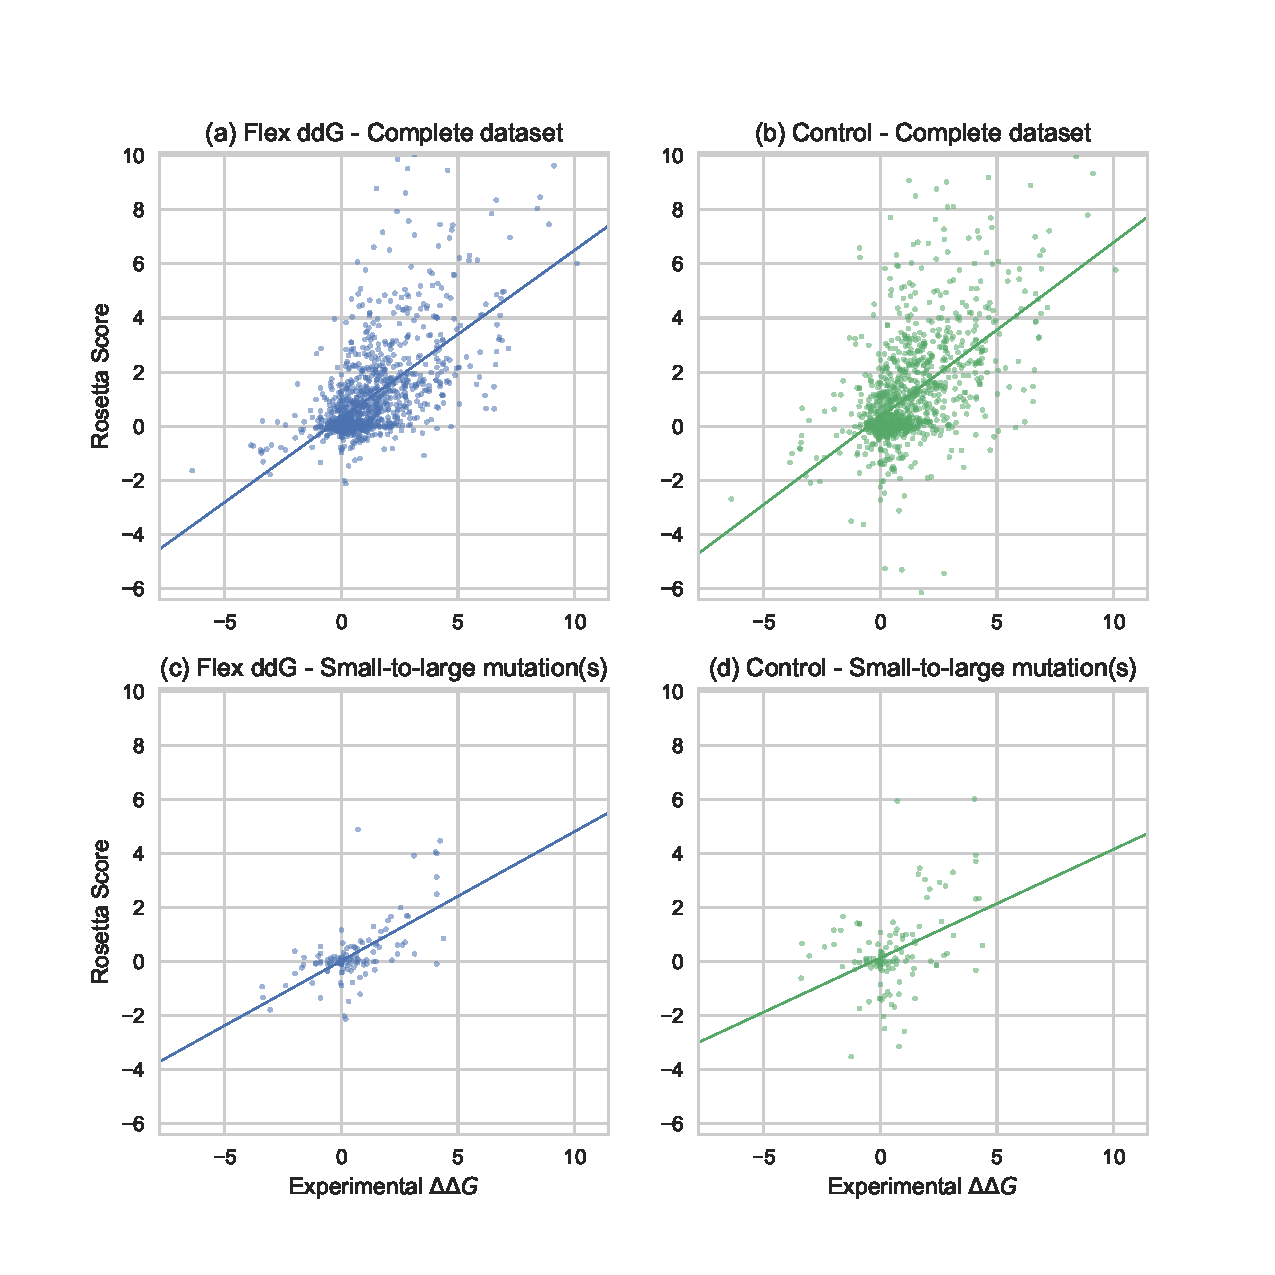
\includegraphics[width=\textwidth,keepaspectratio]{fig-scatter.pdf}
  \caption[]{ % Old subcaption: Rosetta vs. Experimental $\Delta\Delta G$ for flex ddG and no backrub control
    Experimentally determined $\Delta\Delta G$ values (y-axis) vs. Rosetta predictions.
    (a) flex ddG method (35000 backrub steps); Complete dataset mutation set (n=1240).
    (b) no backrub control; Complete dataset mutation set (n=1240).
    (c) flex ddG method (35000 backrub steps); Small-to-large mutation(s) mutation set (n=130).
    (d) no backrub control; Small-to-large mutation(s) mutation set (n=130).
  } \label{fig:figure-scatter}
\end{figure}


% steps-vs-corr figures
\begin{figure}
  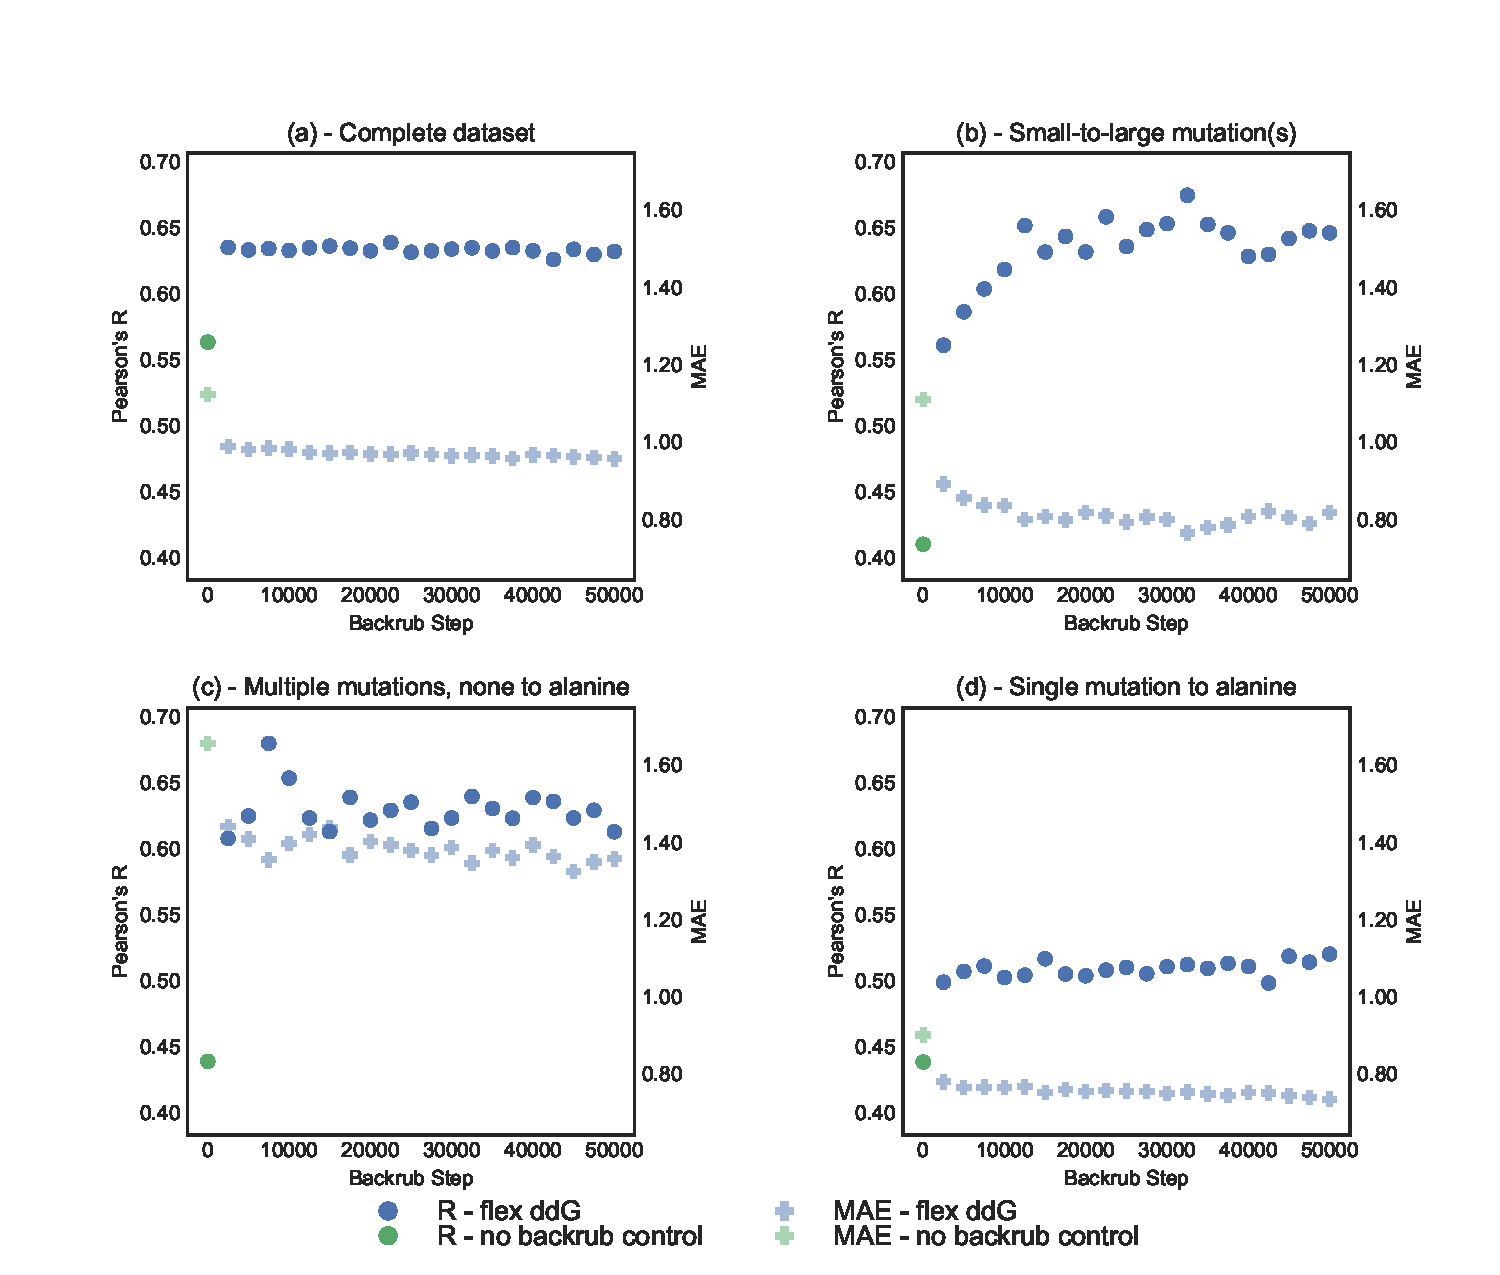
\includegraphics[width=\textwidth,keepaspectratio]{steps-v-corr.pdf}
  \caption[Flex ddG performance vs. number of backrub steps]{
    Correlation (Pearson's R) and MAE (Mean Absolute Error) vs. number of backrub steps, on the complete ZEMu set, and subsets.
    (a) Complete dataset (n=1240)
    (b) Small-to-large mutation(s) (n=130)
    (c) Multiple mutations, none alanine (n=45)
    (d) Single mutation to alanine (n=748)
  } \label{fig:steps-v-corr}
\end{figure}

\begin{figure}
  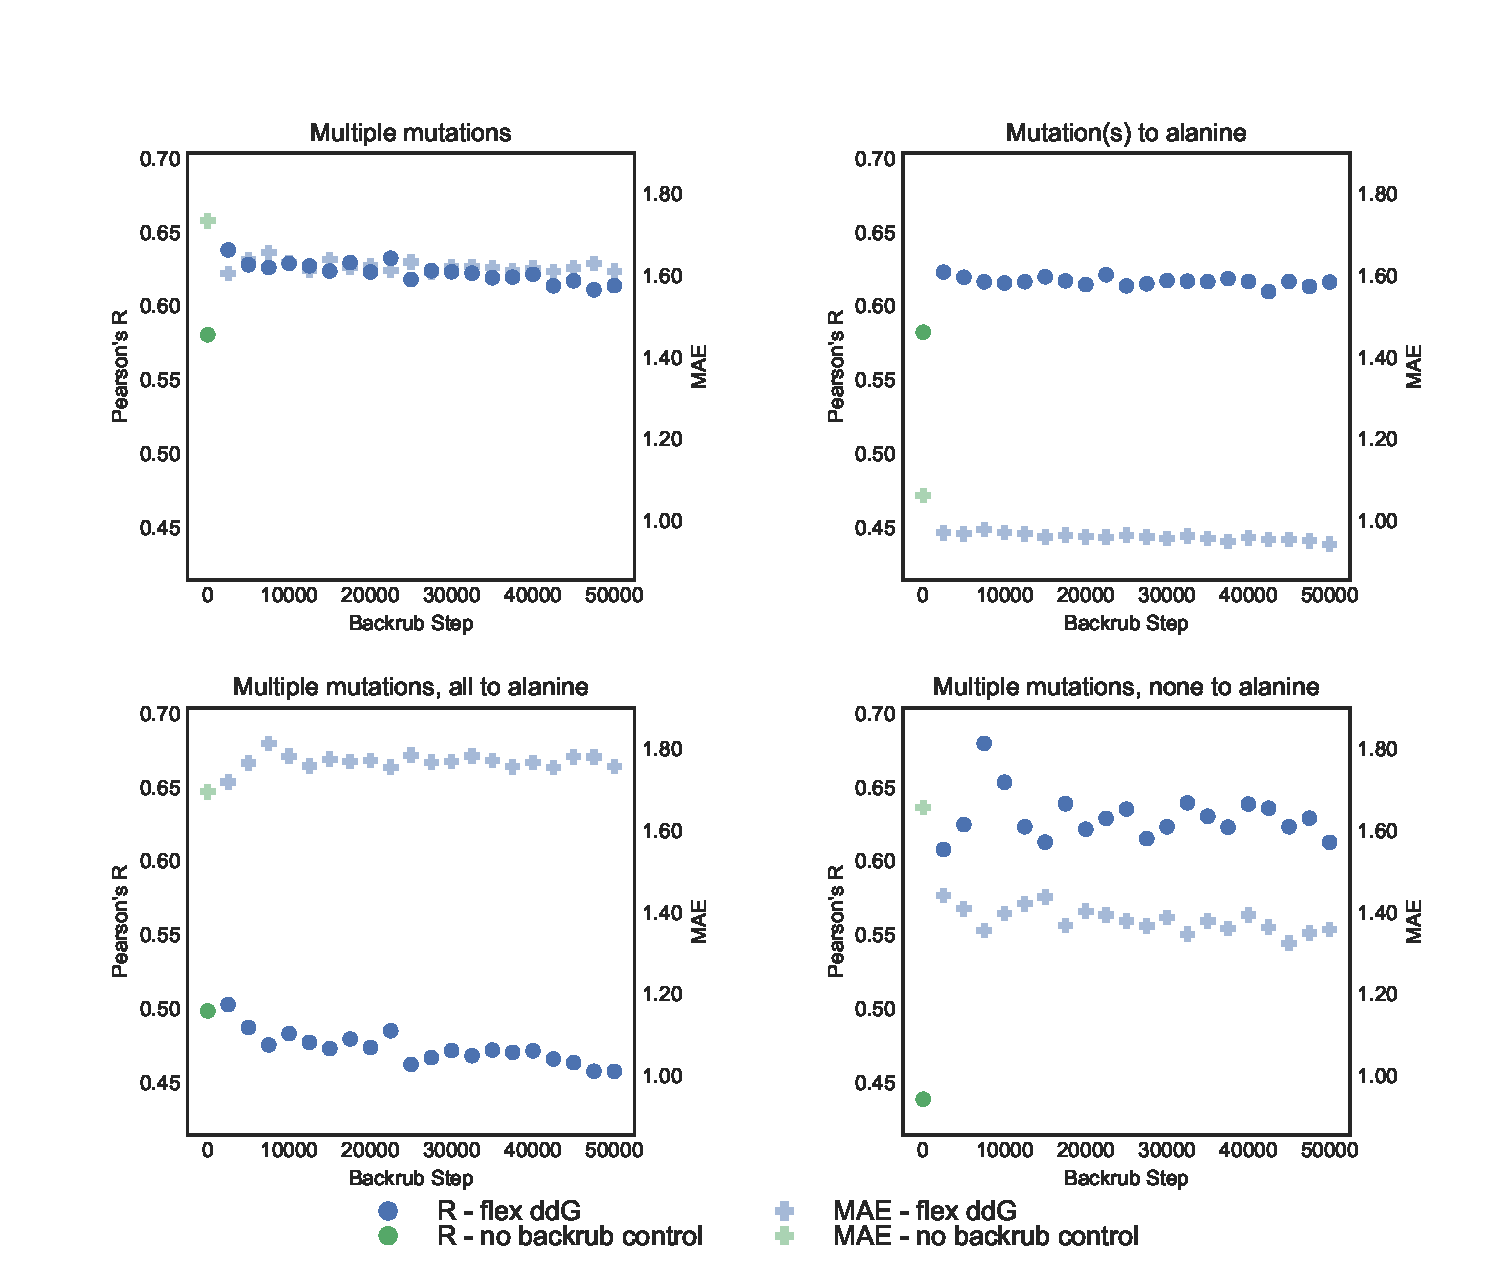
\includegraphics[width=\textwidth,keepaspectratio]{steps-v-corr_mult.pdf}
  \caption[Flex ddG performance vs. number of backrub steps]{
    Correlation (Pearson's R) and MAE (Mean Absolute Error) vs. number of backrub steps, on the complete ZEMu set, and subsets.
    Pearson's R is shown as circles, and MAE as faded plusses.
Predictions generated with the Flex ddG protocol are shown in blue.
Predictions generated with the no backrub control protocol are shown in green.
    A selection of key data underlying this figure can be found in \cref{tab:steps-v-corr_mult-underlying-data}.
    (a) Multiple mutations (n=273)
    (b) Mutation(s) to alanine (n=939)
    (c) Multiple mutations, all to alanine (n=191)
    (d) Multiple mutations, none to alanine (n=45)
  } \label{fig:steps-v-corr_mult}
\end{figure}

\begin{figure}
  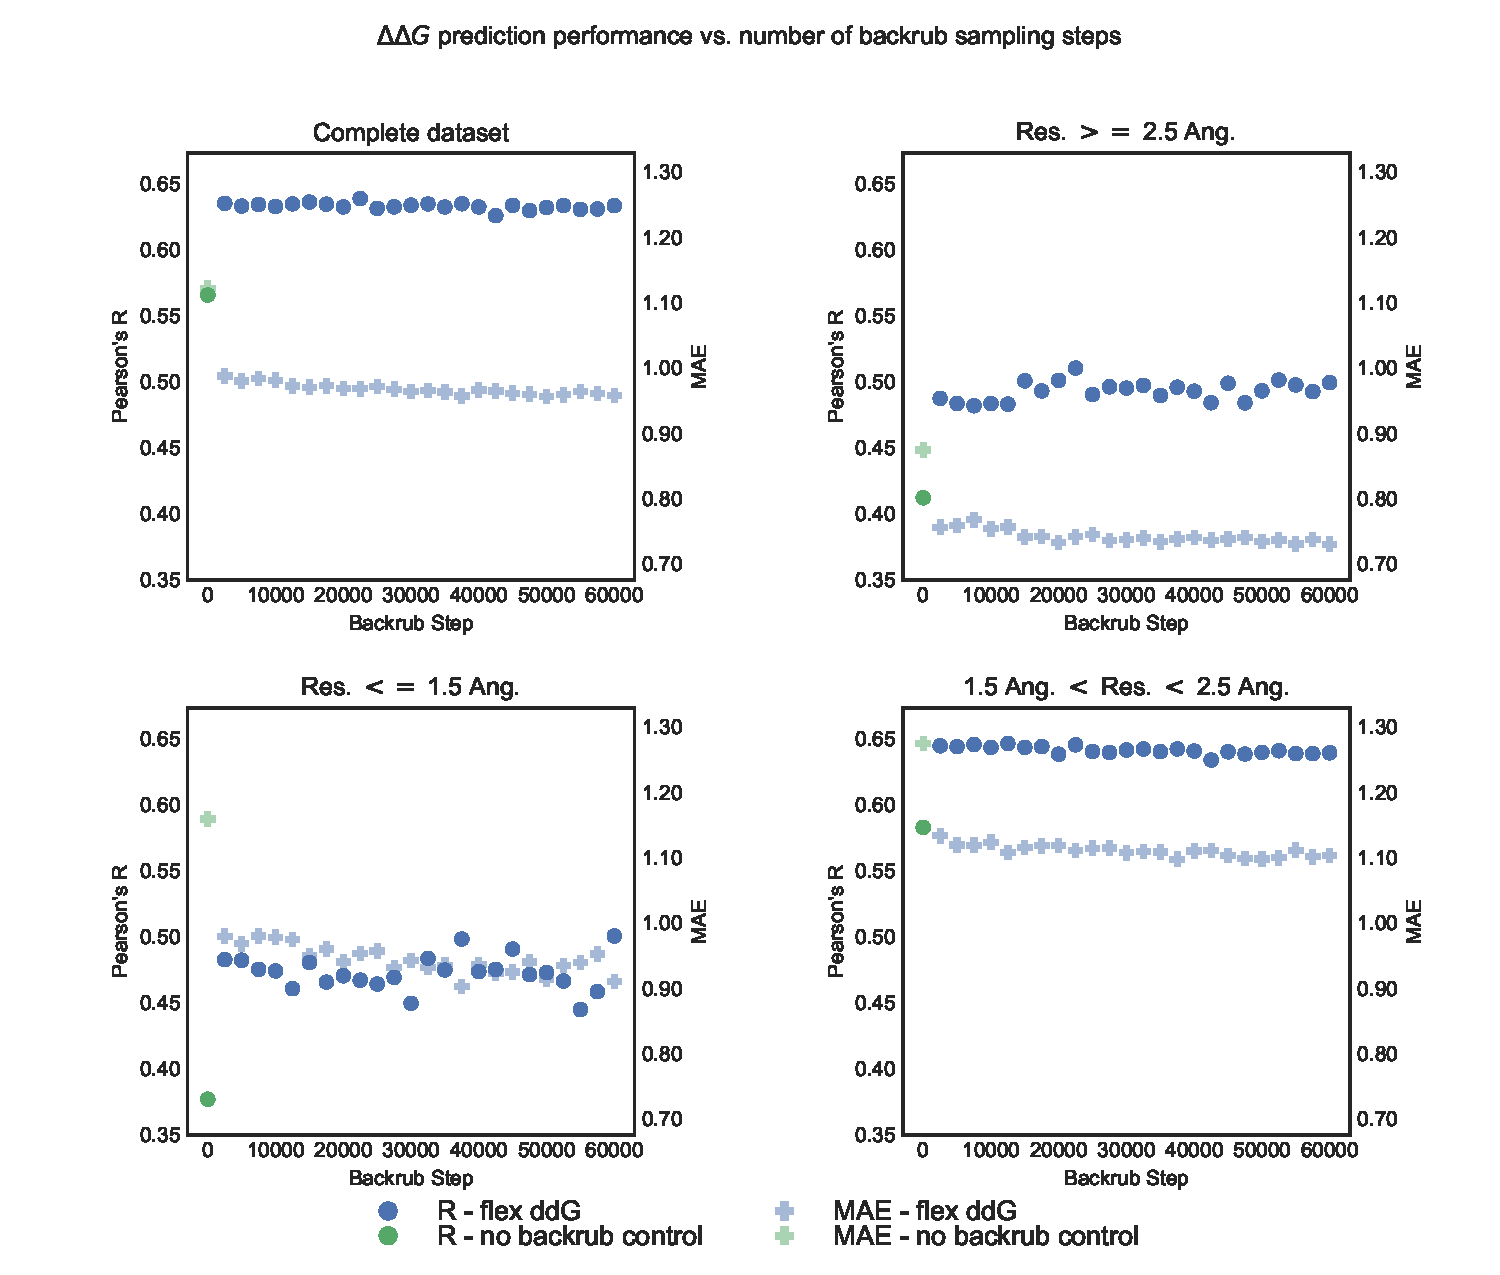
\includegraphics[width=\textwidth,keepaspectratio]{steps-v-corr_resolution.pdf}
  \caption[Flex ddG performance vs. number of backrub steps]{
    Correlation (Pearson's R) and MAE (Mean Absolute Error) vs. number of backrub steps, on the complete ZEMu set, and subsets.
    Pearson's R is shown as circles, and MAE as faded plusses.
Predictions generated with the Flex ddG protocol are shown in blue.
Predictions generated with the no backrub control protocol are shown in green.
    A selection of key data underlying this figure can be found in \cref{tab:steps-v-corr_resolution-underlying-data}.
    (a) (a) - Complete dataset (n=1240)
    (b) (b) - Res. $>=$ 2.5 ang. (n=457)
    (c) (c) - Res. $<=$ 1.5 ang. (n=52)
    (d) (d) - 1.5 ang. $<$ res. $<$ 2.5 ang. (n=731)
  } \label{fig:steps-v-corr_resolution}
\end{figure}

\begin{figure}
  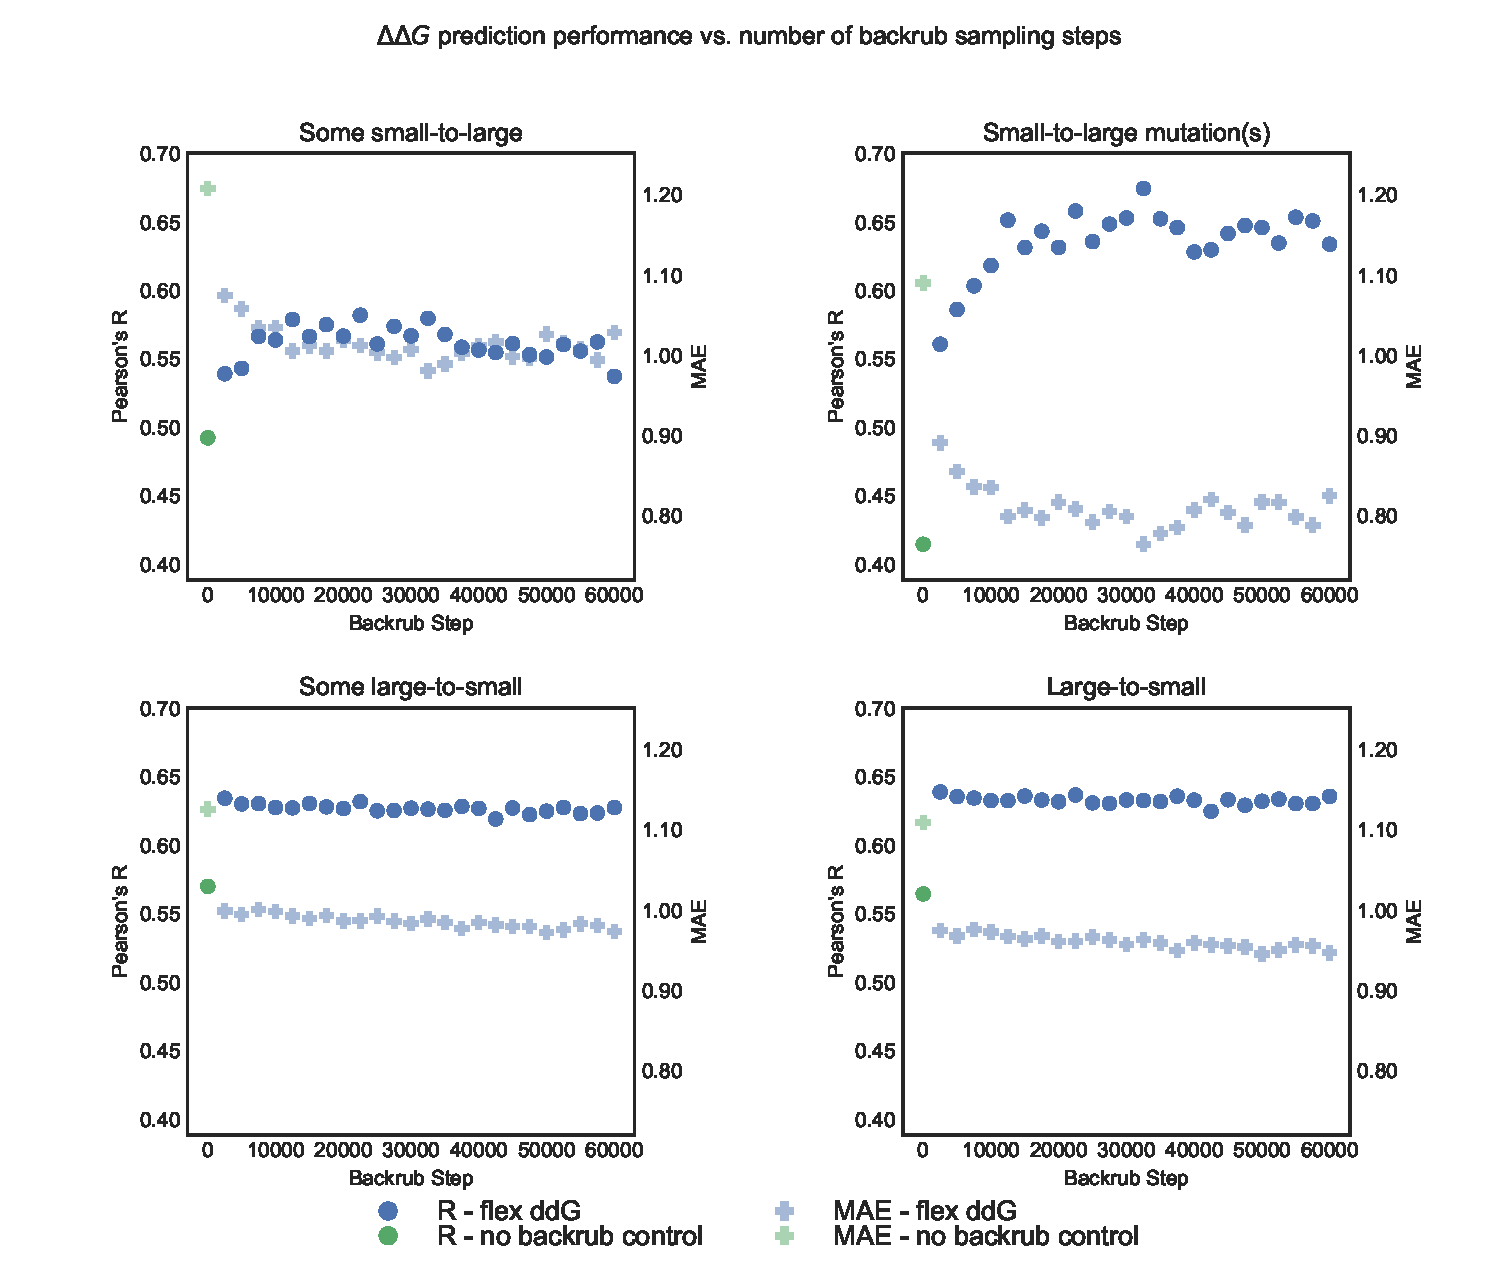
\includegraphics[width=\textwidth,keepaspectratio]{steps-v-corr_some_sizes.pdf}
  \caption[Flex ddG performance vs. number of backrub steps]{
    Correlation (Pearson's R) and MAE (Mean Absolute Error) vs. number of backrub steps, on the complete ZEMu set, and subsets.
    (a) Some small-to-large (n=164)
    (b) Small-to-large mutation(s) (n=130)
    (c) Some large-to-small (n=1110)
    (d) Large-to-small (n=1076)
  } \label{fig:steps-v-corr_some_sizes}
\end{figure}


% structs-vs-corr figures
\begin{figure}
  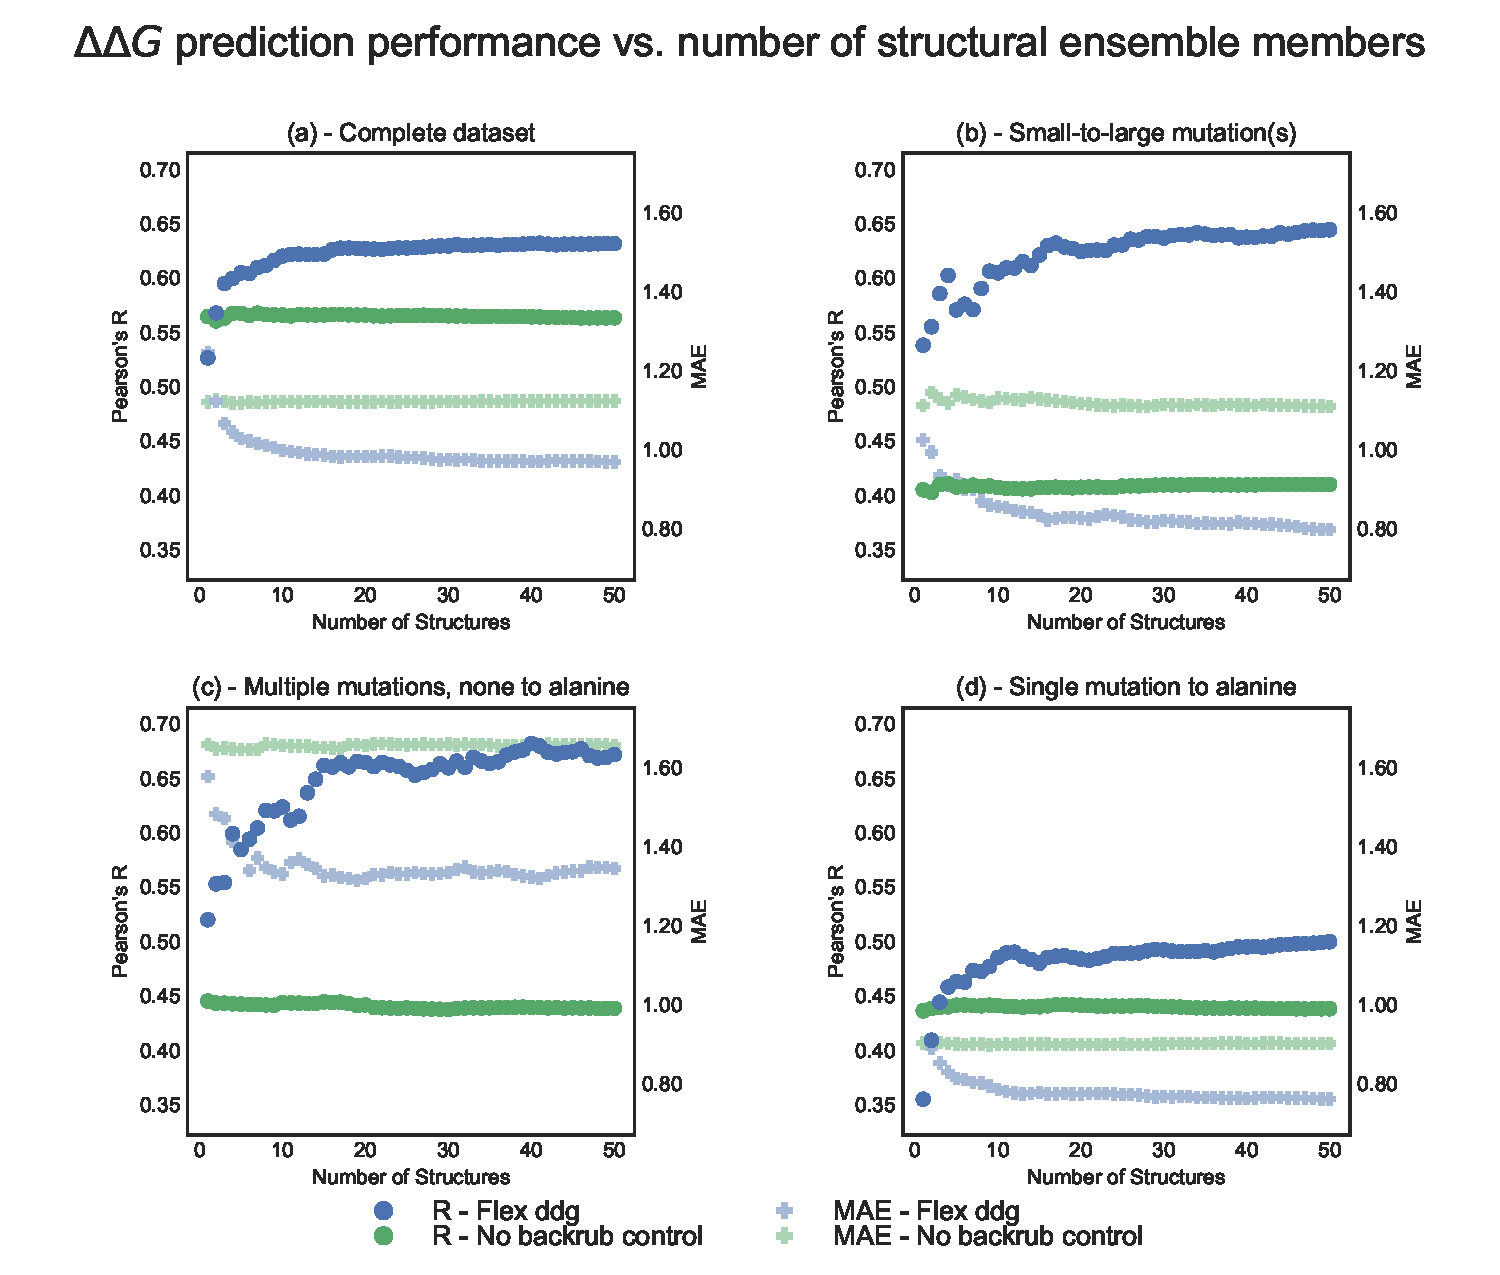
\includegraphics[width=\textwidth,keepaspectratio]{structs-v-corr-id-zemu-12-60000-rscript-validated-t14.pdf}
  \caption[]{ % Old short caption: Flex ddG performance vs. number of averaged structures for flex ddG
    Correlation (Pearson's R, left y-axis) and MAE (Mean Absolute Error, right y-axis) vs. number of averaged structures (x-axis), on the complete ZEMu set, and subsets.
    Pearson's R is shown with circular points, and MAE with faded plus-shaped points.
    Predictions generated with the Flex ddG protocol are shown in blue.
    Predictions generated with the no backrub control protocol are shown in green.
    %% sorting-type%%
    (a) Complete dataset (n = 1240, backrub steps = 35000)
    (b) Small-to-large mutation(s) (n = 130, backrub steps = 35000)
    (c) Multiple mutations, none to alanine (n = 45, backrub steps = 35000)
    (d) Single mutation to alanine (n = 748, backrub steps = 35000)
  } \label{fig:structs-v-corr-id-zemu-12-60000-rscript-validated-t14}
\end{figure}

\begin{figure}
  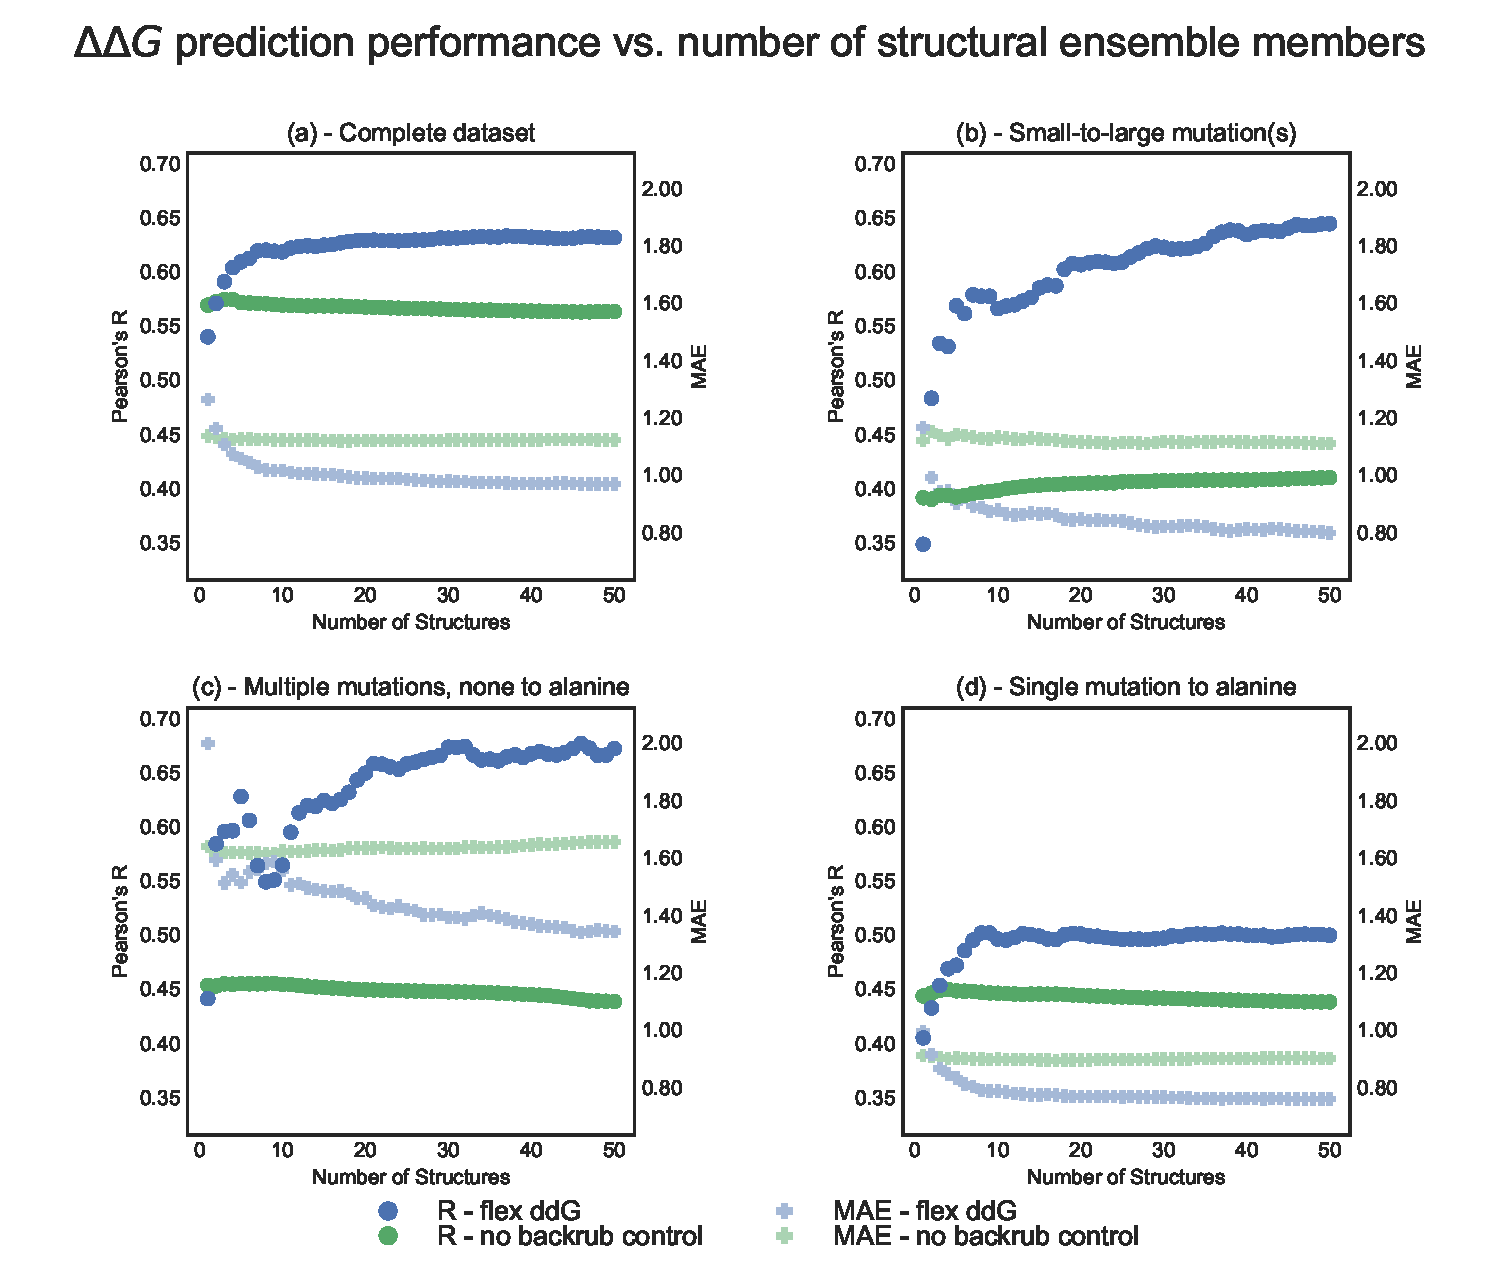
\includegraphics[width=\textwidth,keepaspectratio]{structs-v-corr-WildTypeComplex-zemu-12-60000-rscript-validated-t14.pdf}
  \caption[]{ % Old short caption: Flex ddG performance vs. number of averaged structures for flex ddG
    Correlation (Pearson's R) and MAE (Mean Absolute Error) vs. number of averaged structures, on the complete ZEMu set, and subsets. Structures are sorted by their minimized wild-type complex energy. 
    (a) Complete dataset (n = 1240, backrub steps = 35000)
    (b) Small-to-large mutation(s) (n = 130, backrub steps = 35000)
    (c) Multiple mutations, none alanine (n = 45, backrub steps = 35000)
    (d) Single mutation to alanine (n = 748, backrub steps = 35000)
  } \label{fig:structs-v-corr-WildTypeComplex-zemu-12-60000-rscript-validated-t14}
\end{figure}


\begin{figure}
  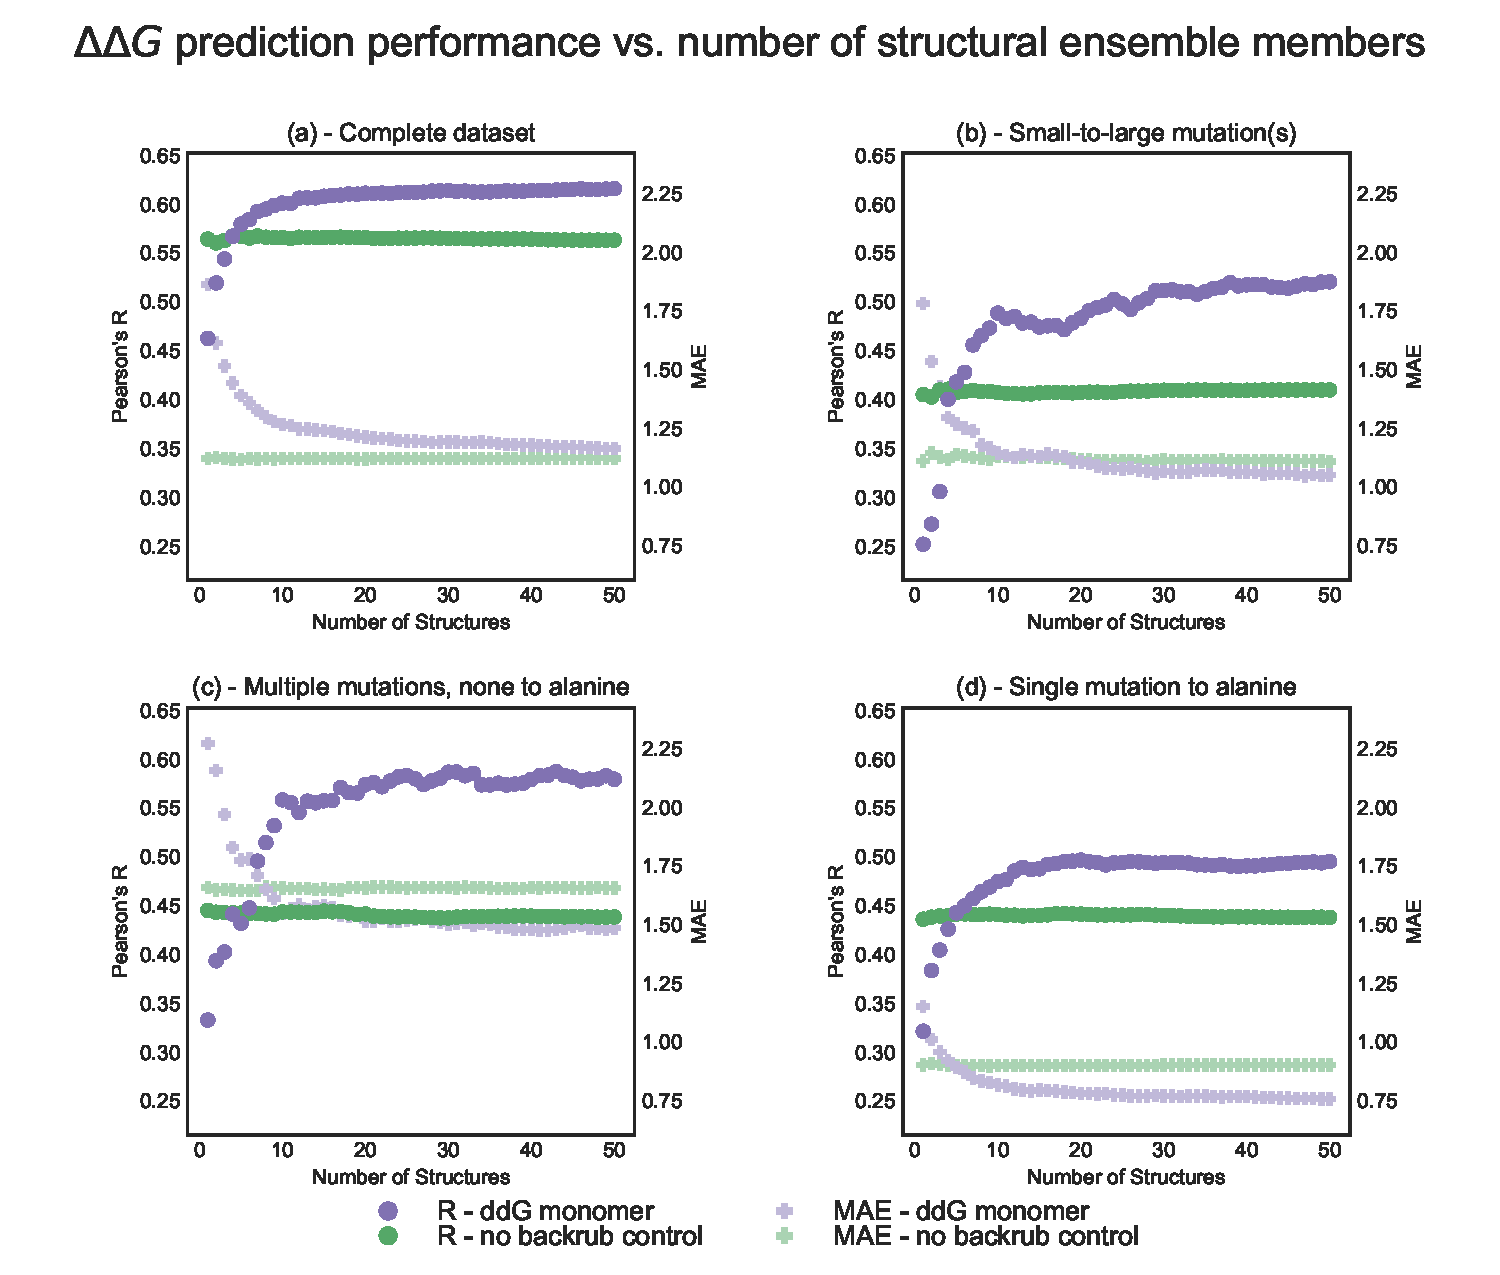
\includegraphics[width=\textwidth,keepaspectratio]{structs-v-corr-id-ddg-monomer-16-003-zemu-2.pdf}
  \caption[]{ % Old short caption: Flex ddG performance vs. number of averaged structures for ddG monomer
    Correlation (Pearson's R) and MAE (Mean Absolute Error) vs. number of averaged structures, on the complete ZEMu set, and subsets. Structures are not sorted, and are randomly added to the ensemble. 
    (a) Complete dataset (n = 1240)
    (b) Small-to-large mutation(s) (n = 130)
    (c) Multiple mutations, none alanine (n = 45)
    (d) Single mutation to alanine (n = 748)
  } \label{fig:structs-v-corr-id-ddg-monomer-16-003-zemu-2}
\end{figure}

\begin{figure}
  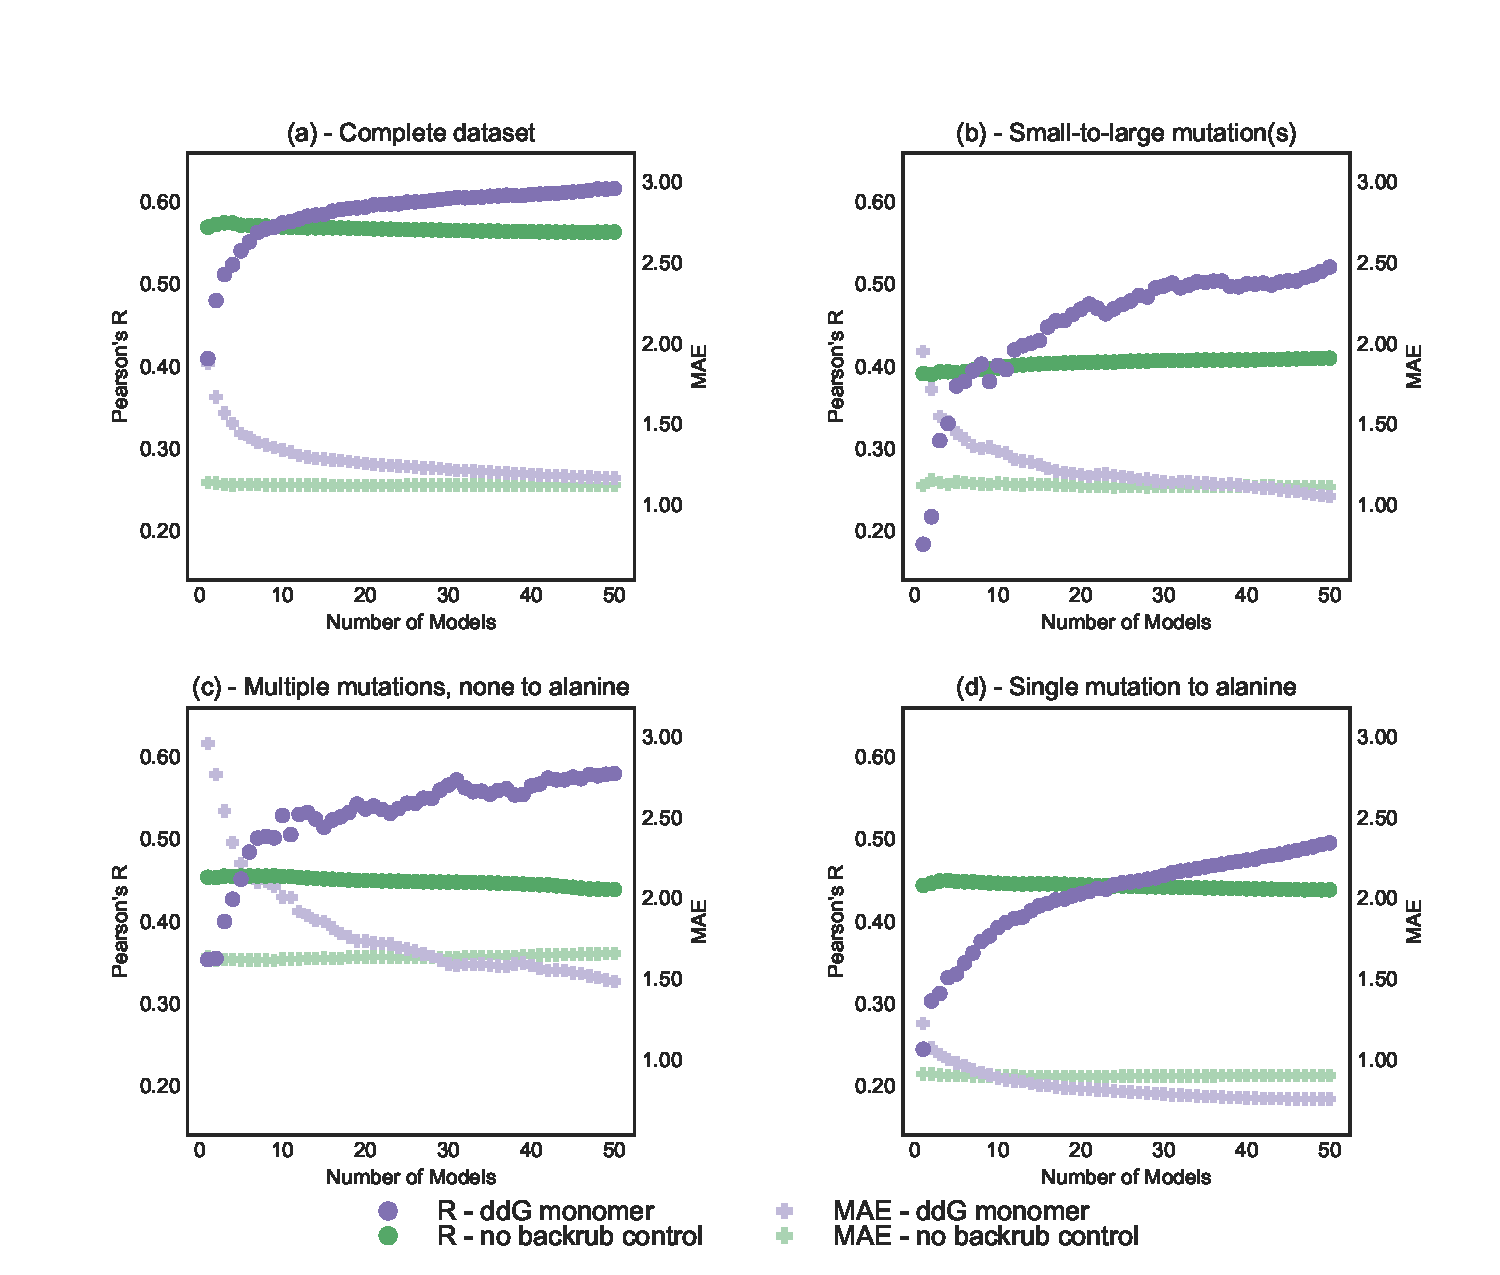
\includegraphics[width=\textwidth,keepaspectratio]{structs-v-corr-WildTypeComplex-ddg-monomer-16-003-zemu-2.pdf}
  \caption[]{ % Old short caption: Flex ddG performance vs. number of averaged structures for ddG monomer
    Correlation (Pearson's R, left y-axis) and MAE (Mean Absolute Error, right y-axis) vs. number of averaged structures (x-axis), on the complete ZEMu set, and subsets.
    Pearson's R is shown with circular points, and MAE with faded plus-shaped points.
    Predictions generated with the ddg\_monomer are shown in purple.
    Predictions generated with the no backrub control protocol are shown in green.
    Data underlying this figure can be found in \cref{tab:structs-v-corr-WildTypeComplex-ddg-monomer-16-003-zemu-2-underlying-data}.
    Structures are sorted by their minimized wild-type complex energy.
    (a) Complete dataset (n = 1240)
    (b) Small-to-large mutation(s) (n = 130)
    (c) Multiple mutations, none to alanine (n = 45)
    (d) Single mutation to alanine (n = 748)
  } \label{fig:structs-v-corr-WildTypeComplex-ddg-monomer-16-003-zemu-2}
\end{figure}


\begin{table}
  \begin{tabular}{llrrrr}
\toprule
Mutation Category &  Prediction Method &     N &    R &  MAE &   FC \\
\midrule
 \multirow{ 2}{*}{Complete dataset} & flex ddG & \multirow{ 2}{*}{1240} & 0.63 & 0.98 & \textbf{0.76}  \\
 & flex ddG (1.6 kT) & & \textbf{0.64} & \textbf{0.93} & 0.75  \\
\hline
 \multirow{ 2}{*}{Small-to-large mutation(s)} & flex ddG & \multirow{ 2}{*}{130} & 0.62 & 0.84 & \textbf{0.72}  \\
 & flex ddG (1.6 kT) & & \textbf{0.64} & \textbf{0.81} & \textbf{0.72}  \\
\hline
 \multirow{ 2}{*}{Single mutation to alanine} & flex ddG & \multirow{ 2}{*}{748} & 0.50 & 0.76 & \textbf{0.75}  \\
 & flex ddG (1.6 kT) & & \textbf{0.51} & \textbf{0.72} & \textbf{0.75}  \\
\hline
 \multirow{ 2}{*}{Multiple mutations} & flex ddG & \multirow{ 2}{*}{273} & \textbf{0.63} & 1.63 & \textbf{0.79}  \\
 & flex ddG (1.6 kT) & & \textbf{0.63} & \textbf{1.52} & 0.75  \\
\hline
 \multirow{ 2}{*}{Multiple mutations, none to alanine} & flex ddG & \multirow{ 2}{*}{45} & \textbf{0.65} & 1.40 & \textbf{0.67}  \\
 & flex ddG (1.6 kT) & & 0.62 & \textbf{1.38} & 0.58  \\
\bottomrule
\end{tabular}
  \caption[Comparison of backrub temperature results]{
    Flex ddG performance comparison, when backrub is run with a sampling temperature (kT) of 1.2 or 1.6 and 10000 backrub steps. N = number of cases in the dataset or subset. R = Pearson's R. MAE = Mean Absolute Error. FC = Fraction Correct. Best performance for each metric is shown in bold.
  } \label{tab:table-temperature}
\end{table}

\begin{table}
  \begin{tabular}{llrrrr}
\toprule
Mutation Category &   Prediction Method &    N &    R &  MAE &   FC \\
\midrule
 \multirow{ 3}{*}{Multiple mutations} & flex ddG & \multirow{ 3}{*}{273} & 0.62 & \textbf{1.62} & \textbf{0.78}  \\
 & no backrub control & & 0.58 & 1.73 & 0.73  \\
 & ZEMu paper & & \textbf{0.64} & 1.63 & 0.75  \\
\hline
 \multirow{ 3}{*}{Multiple mutations, all to alanine} & flex ddG & \multirow{ 3}{*}{191} & 0.47 & 1.77 & \textbf{0.84}  \\
 & no backrub control & & 0.50 & \textbf{1.69} & 0.81  \\
 & ZEMu paper & & \textbf{0.55} & 1.72 & 0.79  \\
\hline
 \multirow{ 3}{*}{Multiple mutations, none to alanine} & flex ddG & \multirow{ 3}{*}{45} & \textbf{0.63} & \textbf{1.38} & \textbf{0.60}  \\
 & no backrub control & & 0.44 & 1.66 & 0.58  \\
 & ZEMu paper & & 0.53 & 1.59 & \textbf{0.60}  \\
\hline
 \multirow{ 3}{*}{Mutation(s) to alanine} & flex ddG & \multirow{ 3}{*}{939} & \textbf{0.62} & \textbf{0.96} & \textbf{0.78}  \\
 & no backrub control & & 0.58 & 1.06 & 0.75  \\
 & ZEMu paper & & \textbf{0.62} & 1.03 & 0.73  \\
\bottomrule
\end{tabular}
  \caption[Multiple mutations results]{
    Multiple mutations results (backrub steps = 35000). N = number of cases in the dataset or subset. R = Pearson's R. MAE = Mean Absolute Error. FC = Fraction Correct.
  } \label{tab:table-mult}
\end{table}

\begin{table}
  \begin{tabular}{llrrrr}
\toprule
Mutation Category &   Prediction Method &     N &    R &  MAE &   FC \\
\midrule
 \multirow{ 4}{*}{Complete dataset} & flex ddG & \multirow{ 4}{*}{1240} & \textbf{0.63} & \textbf{0.96} & \textbf{0.76}  \\
 & no backrub control & & 0.56 & 1.12 & 0.73  \\
 & ddG monomer & & 0.62 & 1.16 & 0.75  \\
 & ZEMu paper & & 0.61 & 1.08 & 0.71  \\
\hline
 \multirow{ 4}{*}{Antibodies} & flex ddG & \multirow{ 4}{*}{355} & \textbf{0.61} & \textbf{0.93} & 0.74  \\
 & no backrub control & & 0.49 & 1.06 & 0.72  \\
 & ddG monomer & & 0.58 & 1.07 & \textbf{0.77}  \\
 & ZEMu paper & & 0.54 & 1.06 & 0.67  \\
\bottomrule
\end{tabular}
  \caption[Flex ddG performance on antibodies]{
    Performance of the Rosetta flex ddG method on the subset of complexes containing an antibody binding partner (flex ddG run with 35000 backrub steps). N = number of cases in the dataset or subset. R = Pearson's R. MAE = Mean Absolute Error. FC = Fraction Correct. Best performance for each metric and dataset is shown in bold.
  } \label{tab:table-antibodies}
\end{table}

\begin{table}
  \begin{tabular}{cl}
    \toprule
    Git SHA1 &                        Protocol \\
    \midrule
    69aa5266f0d5 & flex ddG \\
    69aa5266f0d5 & no backrub control \\
    3b2aa5cc3798 & ddG monomer \\
\bottomrule
\end{tabular}

  \caption{SHA1 Git version of Rosetta used for benchmarking} \label{tab:table-versions}
\end{table}

\begin{table}
  \begin{tabular}{llrrrr}
\toprule
Mutation Category &   Prediction Method &    N &    R &  MAE &   FC \\
\midrule
 \multirow{ 4}{*}{Stabilizing} & flex ddG & \multirow{ 4}{*}{32} & \textbf{0.54} & 2.12 & 0.09  \\
 & no backrub control & & 0.50 & 2.31 & \textbf{0.31}  \\
 & ddG monomer & & 0.39 & 2.18 & 0.19  \\
 & ZEMu paper & & 0.31 & \textbf{2.01} & \textbf{0.31}  \\
\hline
 \multirow{ 4}{*}{Neutral} & flex ddG & \multirow{ 4}{*}{719} & \textbf{0.20} & \textbf{0.51} & \textbf{0.87}  \\
 & no backrub control & & 0.10 & 0.72 & 0.78  \\
 & ddG monomer & & 0.13 & 0.75 & 0.80  \\
 & ZEMu paper & & 0.16 & 0.66 & 0.79  \\
\hline
 \multirow{ 4}{*}{Positive} & flex ddG & \multirow{ 4}{*}{489} & \textbf{0.48} & \textbf{1.55} & 0.63  \\
 & no backrub control & & 0.44 & 1.63 & 0.67  \\
 & ddG monomer & & 0.47 & 1.71 & \textbf{0.72}  \\
 & ZEMu paper & & \textbf{0.48} & 1.63 & 0.62  \\
\bottomrule
\end{tabular}
  \caption[Flex ddG performance on stabilizing mutations]{
    Performance of the Rosetta flex ddG method on the subset of mutations experimentally determined to be stabilizing ($\Delta\Delta G <= -1$), neutral ($-1 < \Delta\Delta G < 1$), or destabilizing ($\Delta\Delta G >= 1$). Flex ddG was run with 35000 backrub steps. N = number of cases in the dataset or subset. R = Pearson's R. MAE = Mean Absolute Error. FC = Fraction Correct.
  } \label{tab:table-stabilizing}
\end{table}

{\small
\begin{longtable}{llrrrr}
\toprule
Mutation Category &   Prediction Method &   N &     R &  MAE &   FC \\
\midrule
 \multirow{ 4}{*}{pdb-1A22} & flex ddG & \multirow{ 4}{*}{142} & \textbf{0.32} & \textbf{0.61} & \textbf{0.79}  \\
 & no backrub control & & 0.18 & 0.77 & 0.74  \\
 & ddG monomer & & 0.12 & 0.91 & 0.73  \\
 & ZEMu paper & & 0.19 & 0.68 & 0.78  \\
\hline
 \multirow{ 4}{*}{pdb-1A4Y} & flex ddG & \multirow{ 4}{*}{45} & 0.81 & 1.34 & 0.71  \\
 & no backrub control & & 0.79 & 1.47 & \textbf{0.78}  \\
 & ddG monomer & & 0.77 & 1.91 & 0.62  \\
 & ZEMu paper & & \textbf{0.87} & \textbf{1.12} & 0.73  \\
\hline
 \multirow{ 4}{*}{pdb-1ACB} & flex ddG & \multirow{ 4}{*}{6} & 0.28 & 2.89 & 0.83  \\
 & no backrub control & & 0.23 & 2.37 & 0.83  \\
 & ddG monomer & & 0.58 & \textbf{1.57} & \textbf{1.00}  \\
 & ZEMu paper & & \textbf{0.79} & 2.17 & 0.83  \\
\hline
 \multirow{ 4}{*}{pdb-1AHW} & flex ddG & \multirow{ 4}{*}{10} & -0.83 & 1.31 & 0.4  \\
 & no backrub control & & -0.42 & 1.42 & 0.4  \\
 & ddG monomer & & -0.34 & 1.26 & 0.5  \\
 & ZEMu paper & & \textbf{0.30} & \textbf{0.93} & \textbf{0.6}  \\
\hline
 \multirow{ 4}{*}{pdb-1AK4} & flex ddG & \multirow{ 4}{*}{15} & \textbf{0.73} & \textbf{0.53} & \textbf{0.73}  \\
 & no backrub control & & 0.35 & 1.01 & 0.47  \\
 & ddG monomer & & 0.63 & 1.35 & 0.60  \\
 & ZEMu paper & & 0.44 & 1.63 & 0.53  \\
\hline
 \multirow{ 4}{*}{pdb-1CBW} & flex ddG & \multirow{ 4}{*}{15} & 0.01 & \textbf{0.59} & \textbf{0.87}  \\
 & no backrub control & & \textbf{0.05} & 0.83 & 0.67  \\
 & ddG monomer & & -0.09 & 0.72 & 0.67  \\
 & ZEMu paper & & -0.26 & 0.71 & 0.67  \\
\hline
 \multirow{ 4}{*}{pdb-1CSE} & flex ddG & \multirow{ 4}{*}{6} & 0.44 & 1.94 & 0.67  \\
 & no backrub control & & 0.37 & 2.03 & 0.67  \\
 & ddG monomer & & 0.46 & 1.88 & 0.67  \\
 & ZEMu paper & & \textbf{0.87} & \textbf{0.81} & \textbf{1.00}  \\
\hline
 \multirow{ 4}{*}{pdb-1DAN} & flex ddG & \multirow{ 4}{*}{118} & 0.65 & \textbf{0.53} & \textbf{0.88}  \\
 & no backrub control & & \textbf{0.69} & 0.59 & 0.85  \\
 & ddG monomer & & 0.61 & 0.71 & 0.83  \\
 & ZEMu paper & & 0.32 & 0.88 & 0.76  \\
\hline
 \multirow{ 4}{*}{pdb-1DFJ} & flex ddG & \multirow{ 4}{*}{20} & 0.70 & 1.35 & \textbf{0.70}  \\
 & no backrub control & & \textbf{0.83} & \textbf{1.04} & 0.60  \\
 & ddG monomer & & 0.69 & 1.38 & 0.55  \\
 & ZEMu paper & & 0.55 & 1.40 & 0.55  \\
\hline
 \multirow{ 4}{*}{pdb-1DQJ} & flex ddG & \multirow{ 4}{*}{34} & \textbf{0.44} & \textbf{1.67} & 0.79  \\
 & no backrub control & & 0.39 & 1.93 & 0.65  \\
 & ddG monomer & & 0.37 & 1.87 & \textbf{0.82}  \\
 & ZEMu paper & & 0.28 & 2.08 & 0.59  \\
\hline
 \multirow{ 4}{*}{pdb-1DVF} & flex ddG & \multirow{ 4}{*}{38} & 0.63 & 1.58 & 0.53  \\
 & no backrub control & & \textbf{0.65} & \textbf{1.50} & 0.66  \\
 & ddG monomer & & 0.61 & 1.54 & \textbf{0.71}  \\
 & ZEMu paper & & 0.57 & 1.54 & 0.53  \\
\hline
 \multirow{ 4}{*}{pdb-1E96} & flex ddG & \multirow{ 4}{*}{6} & \textbf{0.52} & \textbf{0.84} & 0.50  \\
 & no backrub control & & 0.51 & 0.91 & 0.50  \\
 & ddG monomer & & 0.45 & 0.96 & 0.50  \\
 & ZEMu paper & & 0.50 & 0.85 & \textbf{0.67}  \\
\hline
 \multirow{ 4}{*}{pdb-1EAW} & flex ddG & \multirow{ 4}{*}{27} & 0.03 & 0.58 & 0.85  \\
 & no backrub control & & 0.07 & 0.73 & 0.81  \\
 & ddG monomer & & \textbf{0.13} & 0.61 & 0.89  \\
 & ZEMu paper & & 0.00 & \textbf{0.49} & \textbf{0.93}  \\
\hline
 \multirow{ 4}{*}{pdb-1EMV} & flex ddG & \multirow{ 4}{*}{51} & \textbf{0.89} & \textbf{0.86} & \textbf{0.86}  \\
 & no backrub control & & 0.84 & 0.98 & 0.84  \\
 & ddG monomer & & 0.84 & 0.96 & 0.80  \\
 & ZEMu paper & & 0.87 & 0.89 & 0.84  \\
\hline
 \multirow{ 4}{*}{pdb-1F47} & flex ddG & \multirow{ 4}{*}{12} & 0.56 & \textbf{0.72} & 0.50  \\
 & no backrub control & & 0.58 & 0.87 & \textbf{0.58}  \\
 & ddG monomer & & \textbf{0.60} & 0.87 & \textbf{0.58}  \\
 & ZEMu paper & & 0.51 & 1.02 & 0.42  \\
\hline
 \multirow{ 4}{*}{pdb-1FC2} & flex ddG & \multirow{ 4}{*}{9} & -0.07 & \textbf{0.84} & 0.56  \\
 & no backrub control & & -0.09 & 1.01 & 0.67  \\
 & ddG monomer & & -0.39 & 1.19 & 0.44  \\
 & ZEMu paper & & \textbf{0.28} & 0.89 & \textbf{0.78}  \\
\hline
 \multirow{ 4}{*}{pdb-1FCC} & flex ddG & \multirow{ 4}{*}{8} & -0.21 & 1.56 & \textbf{0.5}  \\
 & no backrub control & & -0.22 & 1.96 & \textbf{0.5}  \\
 & ddG monomer & & -0.06 & 1.50 & \textbf{0.5}  \\
 & ZEMu paper & & \textbf{0.16} & \textbf{1.35} & \textbf{0.5}  \\
\hline
 \multirow{ 4}{*}{pdb-1GC1} & flex ddG & \multirow{ 4}{*}{56} & 0.12 & \textbf{0.35} & \textbf{0.91}  \\
 & no backrub control & & -0.15 & 0.43 & 0.86  \\
 & ddG monomer & & 0.28 & 0.38 & 0.86  \\
 & ZEMu paper & & \textbf{0.36} & 0.55 & 0.84  \\
\hline
 \multirow{ 4}{*}{pdb-1HE8} & flex ddG & \multirow{ 4}{*}{10} & 0.39 & 0.67 & \textbf{0.5}  \\
 & no backrub control & & 0.62 & 0.91 & \textbf{0.5}  \\
 & ddG monomer & & 0.26 & \textbf{0.66} & 0.3  \\
 & ZEMu paper & & \textbf{0.81} & 1.23 & \textbf{0.5}  \\
\hline
 \multirow{ 4}{*}{pdb-1IAR} & flex ddG & \multirow{ 4}{*}{36} & 0.64 & \textbf{0.72} & 0.78  \\
 & no backrub control & & 0.35 & 1.32 & 0.67  \\
 & ddG monomer & & \textbf{0.66} & 0.98 & \textbf{0.81}  \\
 & ZEMu paper & & 0.45 & 0.86 & 0.78  \\
\hline
 \multirow{ 4}{*}{pdb-1JCK} & flex ddG & \multirow{ 4}{*}{7} & 0.46 & 1.22 & 0.57  \\
 & no backrub control & & 0.44 & 0.97 & \textbf{0.71}  \\
 & ddG monomer & & 0.75 & 1.25 & \textbf{0.71}  \\
 & ZEMu paper & & \textbf{0.85} & \textbf{0.94} & \textbf{0.71}  \\
\hline
 \multirow{ 4}{*}{pdb-1JRH} & flex ddG & \multirow{ 4}{*}{53} & \textbf{0.58} & \textbf{1.09} & 0.66  \\
 & no backrub control & & 0.50 & 1.25 & 0.60  \\
 & ddG monomer & & 0.52 & 1.29 & \textbf{0.75}  \\
 & ZEMu paper & & 0.57 & 1.15 & 0.58  \\
\hline
 \multirow{ 4}{*}{pdb-1JTG} & flex ddG & \multirow{ 4}{*}{118} & 0.44 & 1.87 & 0.84  \\
 & no backrub control & & 0.39 & \textbf{1.77} & 0.83  \\
 & ddG monomer & & 0.40 & 2.12 & \textbf{0.86}  \\
 & ZEMu paper & & \textbf{0.51} & \textbf{1.77} & 0.75  \\
\hline
 \multirow{ 4}{*}{pdb-1KTZ} & flex ddG & \multirow{ 4}{*}{27} & \textbf{0.86} & \textbf{0.63} & 0.74  \\
 & no backrub control & & 0.76 & 1.16 & \textbf{0.85}  \\
 & ddG monomer & & 0.71 & 1.13 & 0.81  \\
 & ZEMu paper & & 0.80 & 0.83 & 0.70  \\
\hline
 \multirow{ 4}{*}{pdb-1LFD} & flex ddG & \multirow{ 4}{*}{25} & \textbf{0.55} & \textbf{0.68} & \textbf{0.72}  \\
 & no backrub control & & 0.13 & 1.21 & 0.60  \\
 & ddG monomer & & 0.28 & 0.97 & \textbf{0.72}  \\
 & ZEMu paper & & 0.27 & 0.84 & 0.60  \\
\hline
 \multirow{ 4}{*}{pdb-1MLC} & flex ddG & \multirow{ 4}{*}{16} & -0.28 & 1.01 & 0.62  \\
 & no backrub control & & 0.22 & 0.82 & 0.75  \\
 & ddG monomer & & 0.28 & 0.83 & 0.56  \\
 & ZEMu paper & & \textbf{0.79} & \textbf{0.42} & \textbf{0.88}  \\
\hline
 \multirow{ 4}{*}{pdb-1NMB} & flex ddG & \multirow{ 4}{*}{6} & 0.21 & 0.83 & \textbf{0.83}  \\
 & no backrub control & & 0.48 & 0.83 & 0.67  \\
 & ddG monomer & & 0.62 & \textbf{0.60} & \textbf{0.83}  \\
 & ZEMu paper & & \textbf{0.78} & 1.97 & 0.17  \\
\hline
 \multirow{ 4}{*}{pdb-1REW} & flex ddG & \multirow{ 4}{*}{24} & \textbf{0.89} & \textbf{0.67} & \textbf{0.92}  \\
 & no backrub control & & 0.78 & 1.19 & 0.75  \\
 & ddG monomer & & 0.76 & 1.20 & 0.79  \\
 & ZEMu paper & & 0.65 & 1.03 & \textbf{0.92}  \\
\hline
 \multirow{ 4}{*}{pdb-1S1Q} & flex ddG & \multirow{ 4}{*}{6} & 0.17 & \textbf{0.68} & \textbf{0.67}  \\
 & no backrub control & & 0.22 & 0.75 & \textbf{0.67}  \\
 & ddG monomer & & \textbf{0.34} & 0.71 & \textbf{0.67}  \\
 & ZEMu paper & & -0.07 & 1.09 & 0.50  \\
\hline
 \multirow{ 4}{*}{pdb-1TM1} & flex ddG & \multirow{ 4}{*}{21} & 0.33 & 1.71 & 0.43  \\
 & no backrub control & & 0.23 & 1.81 & 0.43  \\
 & ddG monomer & & 0.23 & 1.72 & 0.62  \\
 & ZEMu paper & & \textbf{0.58} & \textbf{1.37} & \textbf{0.71}  \\
\hline
 \multirow{ 4}{*}{pdb-1UUZ} & flex ddG & \multirow{ 4}{*}{5} & 0.79 & 0.62 & \textbf{0.8}  \\
 & no backrub control & & \textbf{0.92} & \textbf{0.52} & \textbf{0.8}  \\
 & ddG monomer & & 0.83 & 0.80 & \textbf{0.8}  \\
 & ZEMu paper & & 0.42 & 1.60 & 0.2  \\
\hline
 \multirow{ 4}{*}{pdb-1VFB} & flex ddG & \multirow{ 4}{*}{43} & 0.58 & \textbf{0.95} & \textbf{0.70}  \\
 & no backrub control & & 0.21 & 1.50 & 0.67  \\
 & ddG monomer & & \textbf{0.64} & 1.40 & \textbf{0.70}  \\
 & ZEMu paper & & 0.60 & 1.07 & 0.65  \\
\hline
 \multirow{ 4}{*}{pdb-1XD3} & flex ddG & \multirow{ 4}{*}{18} & 0.46 & 0.95 & 0.72  \\
 & no backrub control & & 0.28 & 1.43 & 0.67  \\
 & ddG monomer & & 0.51 & 1.15 & 0.67  \\
 & ZEMu paper & & \textbf{0.56} & \textbf{0.71} & \textbf{0.83}  \\
\hline
 \multirow{ 4}{*}{pdb-2I9B} & flex ddG & \multirow{ 4}{*}{5} & -0.81 & 0.53 & \textbf{1.0}  \\
 & no backrub control & & -0.00 & \textbf{0.49} & \textbf{1.0}  \\
 & ddG monomer & & -0.56 & 0.55 & \textbf{1.0}  \\
 & ZEMu paper & & \textbf{0.65} & 0.62 & \textbf{1.0}  \\
\hline
 \multirow{ 4}{*}{pdb-2JEL} & flex ddG & \multirow{ 4}{*}{43} & \textbf{0.67} & 0.64 & \textbf{0.84}  \\
 & no backrub control & & 0.62 & \textbf{0.63} & 0.81  \\
 & ddG monomer & & 0.64 & 0.70 & \textbf{0.84}  \\
 & ZEMu paper & & 0.48 & 0.81 & 0.74  \\
\hline
 \multirow{ 4}{*}{pdb-2PCB} & flex ddG & \multirow{ 4}{*}{6} & \textbf{0.28} & \textbf{0.44} & \textbf{1.00}  \\
 & no backrub control & & 0.23 & 0.64 & 0.67  \\
 & ddG monomer & & -0.70 & 0.90 & \textbf{1.00}  \\
 & ZEMu paper & & -0.63 & 0.95 & 0.83  \\
\hline
 \multirow{ 4}{*}{pdb-2PCC} & flex ddG & \multirow{ 4}{*}{12} & \textbf{0.10} & \textbf{1.27} & \textbf{0.5}  \\
 & no backrub control & & 0.04 & 1.49 & \textbf{0.5}  \\
 & ddG monomer & & -0.29 & 1.90 & \textbf{0.5}  \\
 & ZEMu paper & & -0.24 & 1.53 & \textbf{0.5}  \\
\hline
 \multirow{ 4}{*}{pdb-2VLJ} & flex ddG & \multirow{ 4}{*}{14} & 0.40 & \textbf{0.84} & 0.57  \\
 & no backrub control & & \textbf{0.42} & 1.75 & 0.43  \\
 & ddG monomer & & 0.26 & 0.93 & 0.50  \\
 & ZEMu paper & & 0.15 & 0.89 & \textbf{0.64}  \\
\hline
 \multirow{ 4}{*}{pdb-2WPT} & flex ddG & \multirow{ 4}{*}{32} & 0.54 & 1.60 & 0.62  \\
 & no backrub control & & \textbf{0.63} & \textbf{1.39} & \textbf{0.75}  \\
 & ddG monomer & & 0.56 & 1.63 & 0.69  \\
 & ZEMu paper & & 0.45 & 1.63 & 0.56  \\
\hline
 \multirow{ 4}{*}{pdb-3BK3} & flex ddG & \multirow{ 4}{*}{13} & \textbf{0.72} & \textbf{0.51} & 0.69  \\
 & no backrub control & & 0.70 & 0.98 & 0.62  \\
 & ddG monomer & & 0.65 & 0.55 & \textbf{0.85}  \\
 & ZEMu paper & & 0.31 & 1.45 & 0.54  \\
\hline
 \multirow{ 4}{*}{pdb-3BN9} & flex ddG & \multirow{ 4}{*}{25} & 0.48 & \textbf{0.39} & \textbf{0.88}  \\
 & no backrub control & & \textbf{0.53} & 0.40 & \textbf{0.88}  \\
 & ddG monomer & & 0.31 & 0.66 & \textbf{0.88}  \\
 & ZEMu paper & & -0.09 & 0.66 & 0.84  \\
\hline
 \multirow{ 4}{*}{pdb-3NPS} & flex ddG & \multirow{ 4}{*}{27} & 0.18 & \textbf{0.71} & 0.74  \\
 & no backrub control & & \textbf{0.26} & 0.87 & \textbf{0.78}  \\
 & ddG monomer & & 0.15 & 0.84 & \textbf{0.78}  \\
 & ZEMu paper & & -0.21 & 0.89 & 0.67  \\
\bottomrule
  \caption[Flex ddG performance by PDB structure for all complexes with 5 or more cases]{
    Flex ddG performance by PDB structure for all complexes with 5 or more cases. Backrub steps = 35000. N = number of cases (variants) for each complex. R = Pearson's R. MAE = Mean Absolute Error. FC = Fraction Correct. Best performance for each metric and dataset is shown in bold.
  } \label{tab:table-by-structure}
\end{longtable}

}

\begin{table}
  \begin{tabular}{llrrrr}
\toprule
Mutation Category &      Prediction Method &     N &    R &  MAE &   FC \\
\midrule
 \multirow{ 2}{*}{Complete dataset} & flex ddG & \multirow{ 2}{*}{1240} & \textbf{0.63} & \textbf{0.97} & \textbf{0.76}  \\
 & flex ddG (REF energy) & & \textbf{0.63} & 1.19 & 0.75  \\
\hline
 \multirow{ 2}{*}{Small-to-large mutation(s)} & flex ddG & \multirow{ 2}{*}{130} & \textbf{0.64} & \textbf{0.80} & 0.71  \\
 & flex ddG (REF energy) & & 0.57 & 1.01 & \textbf{0.72}  \\
\hline
 \multirow{ 2}{*}{Single mutation to alanine} & flex ddG & \multirow{ 2}{*}{748} & \textbf{0.50} & \textbf{0.76} & \textbf{0.77}  \\
 & flex ddG (REF energy) & & 0.49 & 0.90 & 0.74  \\
\hline
 \multirow{ 2}{*}{Multiple mutations} & flex ddG & \multirow{ 2}{*}{273} & \textbf{0.62} & \textbf{1.62} & 0.78  \\
 & flex ddG (REF energy) & & 0.59 & 2.12 & \textbf{0.80}  \\
\hline
 \multirow{ 2}{*}{Res. $<=$ 1.5 Ang.} & flex ddG & \multirow{ 2}{*}{52} & 0.46 & \textbf{0.95} & 0.73  \\
 & flex ddG (REF energy) & & \textbf{0.65} & 1.10 & \textbf{0.75}  \\
\hline
 \multirow{ 2}{*}{Res. $>=$ 2.5 Ang.} & flex ddG & \multirow{ 2}{*}{457} & \textbf{0.50} & \textbf{0.74} & \textbf{0.76}  \\
 & flex ddG (REF energy) & & 0.48 & 0.90 & 0.75  \\
\bottomrule
\end{tabular}
  \caption[REF results]{
    Performance comparison of the standard flex ddG protocol (using Rosetta's Talaris energy function) with flex ddG run with the REF score function. "res $<=$ 1.5 Ang." indicates data points for which the resolution of the input wild-type crystal structure is less than or equal to 1.5 \AA. Backrub steps = 35000. R = Pearson's R. MAE = Mean Absolute Error. FC = Fraction Correct. N = number of mutations in the dataset or subset.
  } \label{tab:table-ref}
\end{table}


\end{document}
